\section{Performance Enhancement}


\begin{frame}{A Novel Pre-Processing Method Against Covariate Shift}
    \begin{enumerate}
        \item \textbf{No Prior Shift Knowledge Needed}
        
       
        \item \textbf{Built-in Regularization}
        
    \end{enumerate}
\end{frame}



\begin{frame}{The R.A.W. method}
    \begin{columns}[T]
        \begin{column}{0.35\textwidth}
            \begin{itemize}\LARGE
                \item \textbf{R}andom
                \item \textbf{A}ugmentation
                \item \textbf{W}alk
            \end{itemize}
        \end{column}
        \vline\hspace{1em} 
        
        \begin{column}{0.65\textwidth}
        
    \begin{algorithm}
    \setstretch 
    \begin{algorithmic}
        \STATE \textbf{Input:} $Data_{\text{train}}$, $Size$, $N$, $\varepsilon$.\\[0.5em]
     
        \State $Data_\text{\%}$ \leftarrow $random subset of $N\%$ of $Data$$\\[0.5em]
            \textbf{For} $x_i$ in $Data_\text{\%}$\\[0.5em]
                \State $x_i' \leftarrow 
                \begin{cases}
                    X_i + \varepsilon & \text{with probability } 0.5 \\
                    X_i - \varepsilon & \text{with probability } 0.5
                \end{cases}$\\[0.5em]
                \State $y_i' \leftarrow y_i$\\[0.5em]
            \textbf{End For}\\
            \State $Data_\text{aug} \leftarrow Data_\text{new} \cup Data_\text{\%}$\\[0.5em]
            \State $Data_\text{final} \leftarrow Downsample(Data_\text{aug}, Size)$\\[0.5em]
        \STATE \textbf{Return} $Data_{\text{final}}$
    \end{algorithmic}
    \end{algorithm}
    
          
        \end{column}
    \end{columns}
\end{frame}


\begin{frame}{Classify With Gradient Boosting Using R.A.W.}

\begin{figure}
    \centering
    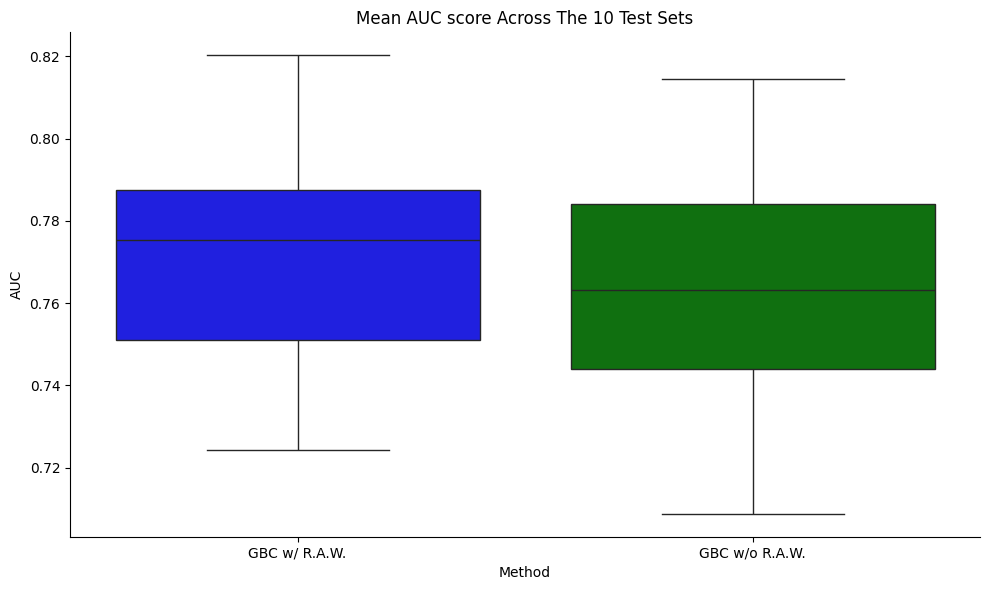
\includegraphics[width=0.45\textwidth]{MeanAUCscoreacross10.png}
    \hfill
    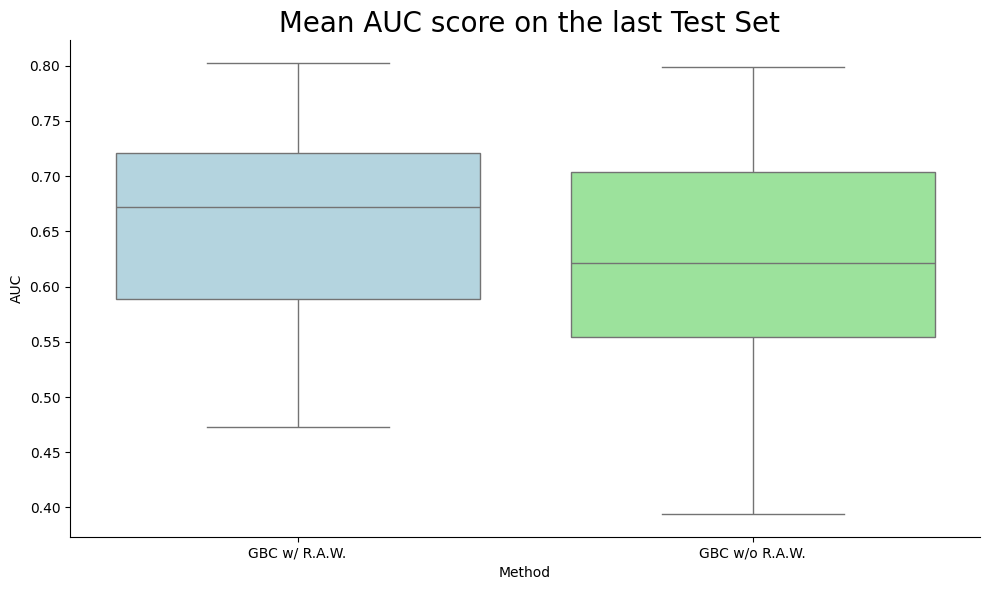
\includegraphics[width=0.45\textwidth]{MeanAUCscoreLAST.png}
\end{figure}




\end{frame}

\begin{frame}{A Statistical Analysis Of The Results}
    \begin{itemize}
        \item \boldsymbol{H_0}:  $\Delta\bar\mu = \overline{AUC}_{R.A.W.} - \overline{AUC}_{base} = 0$
            
            The R.A.W. method does not improve the AUC score of the Gradient Boosting Classifier.
            
        \item \boldsymbol{H_1}: $\Delta\bar\mu = \overline{AUC}_{R.A.W.} - \overline{AUC}_{base}\not= 0$\\
        The R.A.W. method improves the AUC score of the Gradient Boosting Classifier.
        \item \textbf{Test:} Paired t-test on 50 independent $\overline{AUC}$ differences.
    \end{itemize}


        \begin{table}[h!]
            \centering
            \small
            \begin{tabular}{lcccc}
            \hline
            \vspace{1mm}
             & $\bar\Delta\mu$ & t-stat & p-value & 95\% CI \\
            \hline
            \vspace{1mm}
            $\Delta\overline{ AUC}$* & 0.0083 & 8.75  & 1.39e-11 & [0.006, 0.010] \\
            $\Delta\overline{ AUC}_{last}$** & 0.0235 & 10.59 & 2.86e-14 & [0.019, 0.028] \\
            \hline
            \end{tabular}
        \end{table}

    \vspace{1em}
    \begin{footnotesize}
        * Mean AUC score difference across all 10 shifted test sets.\\
        ** Mean AUC score difference on the most shifted test set.
    \end{footnotesize}

\end{frame}

\begin{frame}
    \begin{figure}
        \centering
        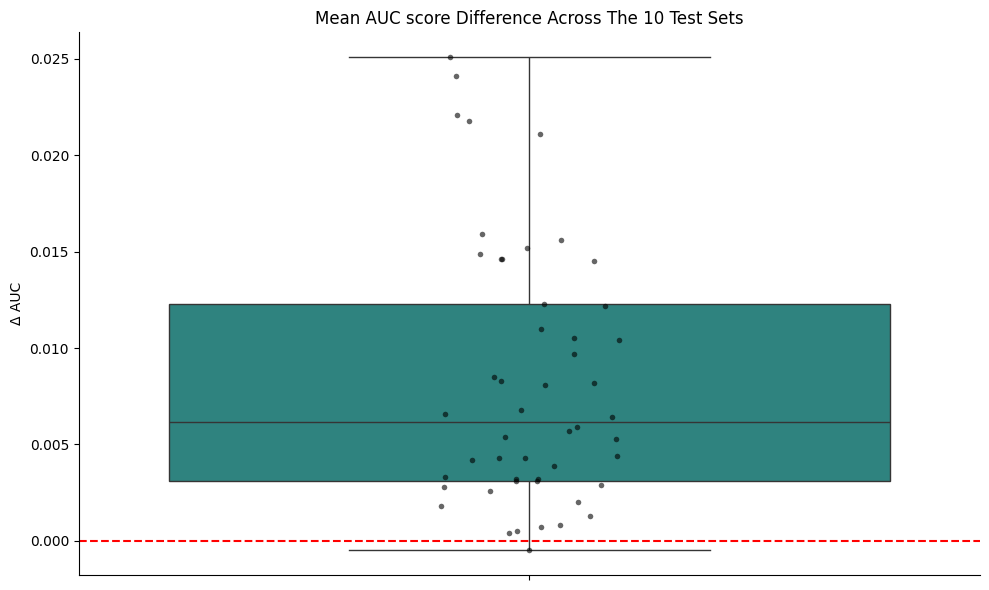
\includegraphics[width=0.45\textwidth]{diffacross10.png}
        \hfill
        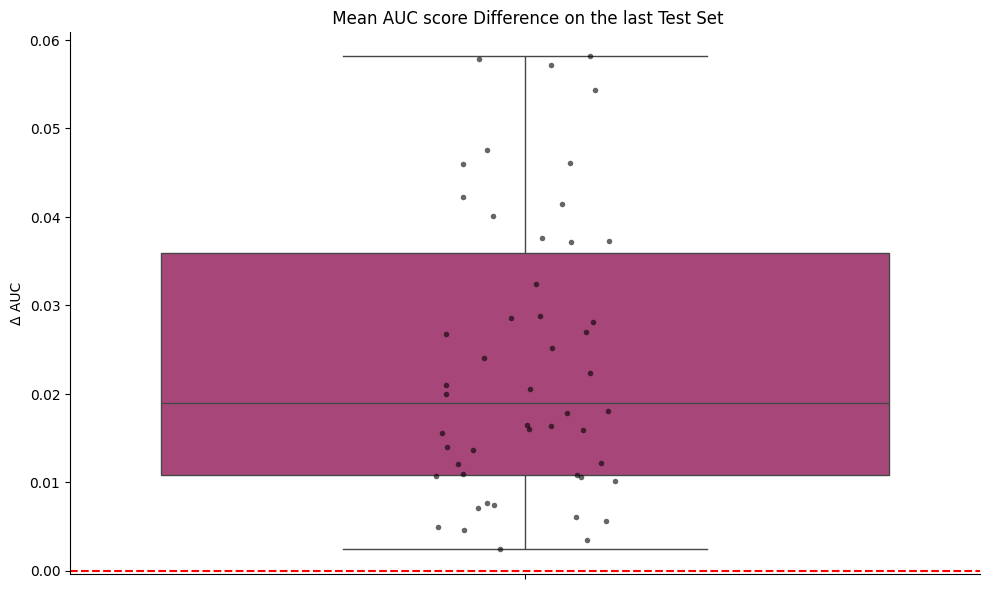
\includegraphics[width=0.45\textwidth]{meandiffLAST.png}
    \end{figure}
\end{frame}

